\section{Software Implementation with SciKit-Surgery}
%these commands might work on some systems if you have -shell-escape set but I couldn't get it working on overleaf
%\immediate\write18{wget https://glenoidplanefitting.readthedocs.io/en/latest/_images/graphviz-f4a0d46f29de525cf2512540ebd2f3e3f3356594.png}
%\input|"wget https://glenoidplanefitting.readthedocs.io/en/latest/_images/graphviz-f4a0d46f29de525cf2512540ebd2f3e3f3356594.png"
\sksglenoid is built on top of the \sksurgery \cite{PMID:32436132} libraries which enabled
rapid development and future deployment into a clinically useable application.
Figure \ref{fig:deps} shows the immediate dependencies of \sksglenoidns.

\begin{figure}
	\begin{center}
		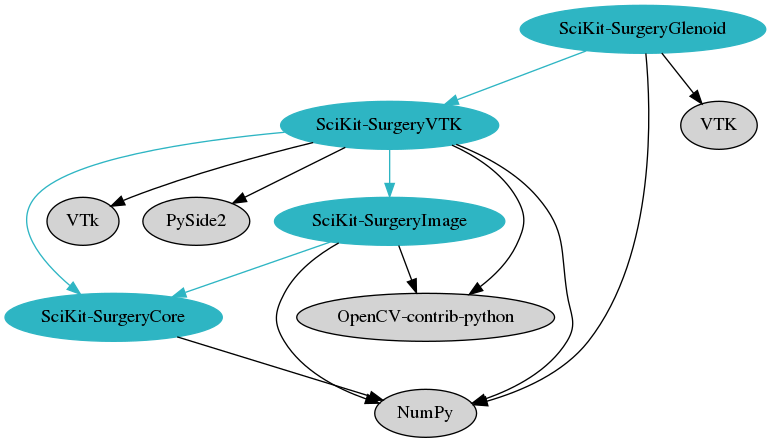
\includegraphics[width=0.6\linewidth]{figures/graphviz-f4a0d46f29de525cf2512540ebd2f3e3f3356594.png}
			\caption{\label{fig:deps}The dependency graph for SciKit-SurgeryGlenoid. SciKit-Surgery dependencies are shown in blue, whilst 3rd party dependencies are shown in grey.}
	\end{center}
\end{figure}
